%Zeilen die mit % anfangen sind Kommentare und werden nicht in der erzeugten Datei angezeigt.
\documentclass[a4paper, 12pt]{scrreprt}
%Legt die Papier und Schriftgröße fest und spezifiziert die Dokumentklasse. Dies findet immer am Anfang jedes Dokuments statt und muss vorhanden sein.

%------------------------------------------------%
%Jetzt werden noch die benötigten Pakete geladen.%
%------------------------------------------------%

\usepackage[colorlinks=true,urlcolor=blue,linkcolor=black,citecolor=black]{hyperref}
%Wird hier nur verwendet um die Links für weitere Informationen einzufügen, kann aber noch sehr viel mehr. Wird vermutlich für die Seminararbeit aber nicht gebraucht.
\usepackage[left=3cm,right=3.5cm,top=3cm,bottom=2.5cm]{geometry}
%Legt die Seitenabstände fest
\usepackage[onehalfspacing]{setspace}
%Legt den Zeilenabstand auf 1.5 fest. Der Zeilenabstand in den Fußnoten wird aber nicht geändert und bleibt bei 1.
\usepackage[ngerman]{babel}
%Ermöglicht das verwenden der deutschen Sonderzeichen und die Silbentrennung nach den neuen deutschen Rechtschreibregeln.
\usepackage{graphicx}
%Ermöglicht es Bilder einzufügen.
\usepackage{pdfpages}
%Ermöglicht es PDF Dateien einzufügen.
\usepackage{amsmath}
%Bietet viele Optionen für den mathematischen Bereich und sollte verwendet werden, wenn mit Formeln gearbeitet wird.
\usepackage{amssymb}
%Stellt weitere Optionen für den mathematischen Bereich zur Verfügung und sollte auch eingebunden werden, wenn mit mathematischen Formeln gearbeitet wird.
\usepackage{MnSymbol}
%Stellt weitere Optionen für den mathematischen Bereich zur Verfügung und sollte auch eingebunden werden, wenn mit mathematischen Formeln gearbeitet wird.
\usepackage{tcolorbox}
%Für farbige Kästen um Text
\usepackage{blindtext}
%Wird eingebunden um Blindtext zu erzeugen, damit die Seminararbeit am Anfang nicht so lehr aussieht. 
\usepackage{biblatex}
%Wird für das Zitieren benötigt.
\addbibresource{Literatur.bib}
%Fügt das Literaturverzeichnis hinzu.

%-----------------------------------------%
%Ab hier beginnt das eigentliche Dokument.%
%-----------------------------------------%

\begin{document}

\begin{titlepage}

\begin{center}
\vspace*{2cm}
{\bfseries\LARGE Test\\} 
\vspace{3cm}
Eine kurze Einführung in das Verfassen von Texten und wissenschaftlichen Arbeiten mit \LaTeX\, .\\
\vspace{4cm}
von Paul Kube
\end{center}

\end{titlepage}

\tableofcontents
\thispagestyle{empty}
\newpage
\setcounter{page}{1}

\chapter{Was brauche ich um mit \LaTeX\, zu arbeiten ?}
\LaTeX\, ist eine sehr mächtige Textsetzungssoftware, mit der sich nicht nur wissenschaftliche Arbeiten, sonder auch Bücher und Folien für Präsentationen erstellen und bearbeiten lassen. Um mit \LaTeX\, arbeiten zu können, benötigt man zuerst einmal eine \LaTeX -Distribution. Es gibt verschiedene \LaTeX\, -Distributionen, die alle verschiedene Möglichkeiten bieten und auf unterschiedlichen Betriebssystemen laufen. Die verbreitetste Distribution für Windows ist MiKTeX (\href{https://miktex.org/}{https://miktex.org/}) und unter MacOS MacTex (\href{https://tug.org/mactex/}{https://tug.org/mactex/}). Eine Übersicht über weitere Distributionen lässt sich bei \href{https://tug.org/interest.html}{https://tug.org/interest.html} unter \glqq 2. Free TeX implementations\grqq\, finden.

Um das Arbeiten mit \LaTeX -Dateien zu vereinfachen empfiehlt es sich einen Editor für \LaTeX\, zu verwenden. TeXworks ist ein solcher Editor, der auch gleich in MiKTeX und MacTex enthalten ist. Mir persönlich gefällt der Editor TeXmaker (\href{https://www.xm1math.net/texmaker/}{https://www.xm1math.net/texmaker/}) besser. Dieser muss jedoch zusätzlich installiert werden. Eine Liste weiterer Editoren für \LaTeX\, ist bei \href{https://tug.org/interest.html}{https://tug.org/int\\erest.html} unter \glqq 3. TeX engines and extensions\grqq\, zu finden.
 
\chapter{Aufbau einer \LaTeX -Datei}
Das Aussehen und der Aufbau von \LaTeX -Dateien ist grundlegend anders als der von Word-Dateien. Während bei Word die fertige Datei genauso aussieht wie die zuvor in Word geschriebene Datei, ist dies bei \LaTeX-Dateien nicht der Fall. Diese enthalten Befehle, die den Text verändern aber selber in der fertigen Datei nicht mehr zu finden sind. Dadurch ist der Einstieg etwas gewöhnungsbedürftig und es braucht etwas Zeit um sich an die neue Umgebung zu gewöhnen. Dieser Text soll den Einstieg in das Arbeiten mit \LaTeX\, vereinfachen und Orientierung für den Anfang bieten.\\

\section{Grundstruktur einer \LaTeX -Datei}
Zu Beginn soll der grundlegende Aufbau jeder .tex\textbackslash \LaTeX -Datei geklärt werden. Am Anfang jeder .tex Datei steht immer der Befehl\\ 
\hspace*{0.5cm}\textbf{\textbackslash documentclass[Optionen]\{Dokumentklasse\}}.\\
Zwischen den eckigen Klammern können Optionen für das Layout festgelegt werden, zum Beispiel mit a4paper die Seitengröße auf A4. Auch die Schriftgröße lässt sich mit 12pt auf die Schriftgröße 12 festlegen. 

Für die Dokumentklasse gibt es viele verschiedene Optionen, alle mit unterschiedlichen Möglichkeiten und Anwendungsbereichen. Für die Seminararbeit empfiehlt es sich den Dokumentklasse scrreprt zu verwenden.

Weitere Informationen über den Befehl \textbackslash documentclass, sowie die verschiedenen Optionen und möglichen Dokumenttypen sind hier \href{https://de.wikibooks.org/wiki/LaTeX-W\%C3\%B6rterbuch:_documentclass}{https://de.wikibooks.org/\\wiki/LaTeX-Wörterbuch:\_documentclass}  und eine ausführliche Liste über alle Dokumentklassen hier \href{https://www.namsu.de/Extra/latex-klassen.html}{https://www.namsu.de/Extra/latex-klassen.html} zu finden.\\

\noindent Anschließend wird mit dem Befehl \textbf{\textbackslash begin\{document\}} das eigentliche Dokument begonnen und am Ende mit dem Befehl \textbf{\textbackslash end\{document\}} beendet.\\
\newpage
Somit sieht das kleinst mögliche \LaTeX -Dokument so aus:\\
\begin{addmargin}{0.5cm}
\textbackslash documentclass\{scrreprt\}\\
\textbackslash begin\{document\}\\
\textbackslash end\{document\}\\
\end{addmargin}

\noindent Der Bereich zwischen \textbackslash documentclass\{article\} und \textbackslash begin\{document\} wird Prä-\\ambel genannt und ist dafür da weiter Pakete einzubinden oder eigene Definitionen festzulegen. Weitere Pakete lassen sich mit dem Befehl \textbf{\textbackslash usepackage\{Paket\\name\}} einbinden. \LaTeX\, enthält von sich aus schon viele Optionen, jedoch werden vor allem für mathematische Formeln oder für das Zitieren weitere Pakete benötigt.\\
Für die Seminararbeit empfiehlt es sich folgende Pakete einzubinden:\\
\begin{itemize}
\item \textbackslash usepackage[left=3cm,right=3.5cm,top=3cm,bottom=2.5cm]\{geometry\}\\
Legt die Seitenabstände fest.
\item \textbackslash usepackage[onehalfspacing]\{setspace\}\\
Legt den Zeilenabstand auf 1.5 fest. Der Zeilenabstand in den Fußnoten wird aber nicht geändert und bleibt bei 1.
\item \textbackslash usepackage[ngerman]\{babel\}\\
Ermöglicht das verwenden der deutschen Sonderzeichen und die Silbentrennung nach den neuen deutschen Rechtschreibregeln.
\item \textbackslash usepackage\{graphicx\}\\
Ermöglicht es Bilder einzufügen.
\item \textbackslash usepackage\{pdfpages\}\\
Ermöglicht es PDF Dateien einzufügen.
\item \textbackslash usepackage\{amsmath\}\\
Bietet viele Optionen für den mathematischen Bereich und sollte verwendet werden, wenn mit Formeln gearbeitet wird.
\item \textbackslash usepackage\{amssymb\}\\
Stellt weitere Optionen für den mathematischen Bereich zur Verfügung und sollte auch eingebunden werden, wenn mit mathematischen Formeln gearbeitet wird.
\item \textbackslash usepackage\{MnSymbol\}\\
Stellt weitere Optionen für den mathematischen Bereich zur Verfügung und sollte auch eingebunden werden, wenn mit mathematischen Formeln gearbeitet wird.
\item \textbackslash \{tcolorbox\}\\
Ermöglicht es farbige Kästen um Text zu erzeugen.
\item \textbackslash usepackage\{blindtext\}\\
Wird eingebunden um Blindtext zu erzeugen, damit die Seminararbeit am Anfang nicht so leer aussieht. 
\item \textbackslash usepackage\{biblatex\}\\
Wird für das Zitieren benötigt.
\end{itemize}
Diese Pakete sollten für den Start reichen und werden für die in diesem Text besprochenen Befehle benötigt. Eine genauere Übersicht über die genannten Pakete, sowie über viele weitere lässt sich auf dieser Website  \href{https://www.namsu.de/Extra/latex-pakete.html}{https://www.namsu.de/Extra\\/latex-pakete.html} finden.

\section{Erstellen einer Titelseite und Inhaltsverzeichnis und anpassen der Seitenzahlen}
\hspace*{0.5cm}Um eine Titelseite zu erstellen, hat man zwei Optionen. Man kann entweder in der Präambel mit den Befehlen \textbf{\textbackslash title \textbackslash autor} den Titel und den Autor festzulegen und dann im Dokument mit dem Befehl \textbf{\textbackslash maketitle} die von \LaTeX\, vordefinierte Titelseite zu erzeugen. Oder man gestaltet zwischen den Befehlen \textbf{\textbackslash begin\{titlepage\}} und \textbf{\textbackslash end\{titlepage\}} die Titelseite selber. Mehr Infos zum gestalten einer Titelseite findet man, indem man in die .tex Datei dieses PDFs schaut oder auf der Webseite \href{https://de.wikibooks.org/wiki/LaTeX/_Eine_Titelseite_erstellen}{https://de.wikibooks.org/wiki/LaTeX/\_Eine\_Titel\\seite\_erstellen}.\\

Das Erstellen eines Inhaltsverzeichnissen mit \LaTeX\, ist sehr simple. Man muss lediglich den Befehl \textbf{\textbackslash tableofcontents} an der gewünschten Stelle einfügen. Dieser erzeugt aus den einzelnen sections und subsections, auf die im Kapitel 3 eingegangen wird, das Inhaltsverzeichnis. Damit Änderungen im Inhaltsverzeichnis erscheinen, muss die Datei zwei mal übersetzt werden.\\

\LaTeX\, fügt automatisch die Seitenzahlen unten in der Mitte ein. Möchte man auf einer Seite zum Beispiel bei dem Inhaltsverzeichnis die Seitenzahl unterdrücken, verwendet man den Befehl \textbf{\textbackslash thispagestyle\{empty\}}. Danach sollte aber mit \textbf{\textbackslash newpage} eine neue Seite erzeugen. Will man die Seitenzahl verändert, verwendet man \textbf{\textbackslash setcounter\{page\}\{1\}}, um die Seitenzahl der aktuellen Seite z.B. auf 1 zu setzen.\\
Der Anfang der Seminararbeit nach \textbackslash begin\{document\} könnte demnach so aussehen:\\
\begin{addmargin}{0.5cm}
\textbackslash begin\{document\}\\
\hfill\\
\textbackslash begin\{titlepage\}\\
\hfill\\
Hier Titelseite gestalten\\
\hfill\\
\textbackslash end\{titlepage\}\\
\hfill\\
\textbackslash tableofcontents\\
\textbackslash thispagestyle\{empty\}\\
\textbackslash newpage\\
\textbackslash setcounter\{page\}\{1\}\\
\end{addmargin}
Damit wird die Titelseite und das Inhaltsverzeichnis erzeugt und die Seitenzahlen beginnen auf der erste Seite.

\chapter{Fließtexte schreiben und bearbeiten}
\section{Überschriften}
Die Überschriften werden, wie in dem Vorherigen Kapitel erwähnt, automatisch in das Inhaltsverzeichnis eingefügt. In der Klasse scrreprt ist die Struktur der Überschriften und Unterüberschriften wie folgt:
\begin{itemize}
\item \textbf{\textbackslash chapter\{Kapitelname\}} für die einzelnen Kapitel in der Seminararbeit
\item \textbf{\textbackslash section\{Überschrift\}} für die einzelnen Überschriften in den Kapiteln
\item \textbf{\textbackslash subsection\{Unterüberschrift\}} für Unterüberschriften
\end{itemize}
Zwischen den geschweiften Klammern steht die Überschrift, diese wird von \LaTeX\, automatisch größer und fett geschrieben. Die Größe der Überschrift ist abhängig davon, ob es ein chapter oder eine section ist, wobei ein chapter die größte Überschrift darstellt. Zudem beginnt jedes chapter auf einer neuen Seite. 

\section{Text bearbeiten \\(Schriftgröße und Art, fett, unterstreichen)}
\begin{tabular}{ll}
\textbf{\textbackslash Huge} & {\huge Riesig}\\
\textbf{\textbackslash tiny} & {\tiny winzig}\\
\textbf{\textbackslash texttt\{ \}} & \texttt{Schreibmaschine}\\
\textbf{\textbackslash textit\{ \}} & \textit{Kursiv}\\
\textbf{\textbackslash textbf\{ \}} & \textbf{fett}\\
\textbf{\textbackslash underline\{ \}} & \underline{unterstrichen}\\
\end{tabular}\hfill\\
Weitere Informationen zur Textgröße und den anderen Befehlen,  befinden sich auf dieser Internetseite \href{https://www.namsu.de/latex/kapitel5_1.html}{https://www.namsu.de/latex/kapitel5\_1.html}

\section{Text hervorheben}
Hier werden zwei weitere Methoden neben dem fett schreiben gezeigt, mit denen sich Textstellen hervorheben lassen.\\
Mit der Umgebung \textbf{\textbackslash begin\{tcolorbox\}} lässt sich Text in einen farbigen Kasten schreiben.
\begin{addmargin}{0.5cm}
\textbackslash begin\{tcolorbox\}\\
Dieser Text sticht hervor!\\
\textbackslash end\{tcolorbox\}\\
\end{addmargin}
\begin{tcolorbox}
Dieser Text sticht hervor!
\end{tcolorbox}
Eine andere Möglichkeit ist der Befehl \textbf{\textbackslash emph\{ Hervorzuhebender Text\}}, welcher dieses Ergebnis liefert:\\
\hspace*{0.5cm}Hier kommt jetzt ein Text in dem \emph{diese Stelle hervorgehoben} werden soll.

\section{Absätze, Abstände und Einrückungen}
Absätze, Abstände und Einrückungen werden nicht aus der .tex Datei übernommen, sondern mit Befehlen erzeugt.

Für einen Zeilenumbruch verwendet man den Befehl \textbf{\textbackslash \textbackslash}. 
Möchte man einen neuen Absatz haben, kann man entweder \textbf{\textbackslash par} verwenden oder eine Lehrzeile in der .tex Datei lassen.
Hier kommt ein Test zu der Funktionsweise von \textbackslash par, wie sieht so ein Absatz aus?\par
Jetzt geht es weiter nachdem \textbackslash par Befehl so sieht so ein Absatz also aus. Verbindet man nun einen Zeilenumbruch und einen Neuen Absatz, so sieht das entsprechende Ergebnis so aus.\\

Hier geht es jetzt Weiter nach einem Zeilenumbruch und einem Absatz. Wie man sieht entsteht ein Abstand zu dem neuen Absatz. Wie auch schon bei dem einfachen Absatz ist dieses mal wieder die neue Zeile zu beginn eingerückt. Dies ist gängiger Stil möchte man dies jedoch trotzdem vermeiden, verwendet man am Anfang der folgenden Zeile \textbackslash noindent \\ \par
\noindent Das Ergebnis sieht dann so aus. Hierfür wurde wieder ein Zeilenumbruch zusammen mit einem neuen Absatz verwendet, um den Effekt zu verdeutlichen.\\
Um ganze Textabsätze einzurücken, gibt es die Umgebung\\
\hspace*{0.5cm} \textbf{\textbackslash begin\{addmargin\}\{Weite der Einrückung von Links\}}.\\ Als Beispiel zur Veranschaulichung ist der nächste Absatz zwischen den Befehlen \textbf{\textbackslash begin\{addmargin\}\{3cm\}} und \textbf{\textbackslash end\{addmargin\}} geschrieben.
\begin{addmargin}{1cm}
\blindtext
\end{addmargin}

\noindent Der hier verwendete Absatz ist ein Blindtext, der in \LaTeX\, mit dem Befehl \textbf{\textbackslash blindtext} eingefügt werden kann. Mit weiteren Optionen lassen sich mit diesem Befehl auch ganze Seiten Blindtext einfügen. Alle Informationen zu dem Befehl sind hier \href{http://tex.lickert.net/packages/blindtext/}{http://tex.lickert.net/packages/blindtext/} zu finden. Blindtext bietet sich besonders zu Beginn des Schreibens der Seminararbeit an, um den leeren Platz zwischen den einzelnen Überschriften zu füllen.

\section{Sonderzeichen}
In \LaTeX\, sind eine Liste von Sonderzeichen wie zum Beispiel \textbf{\textbackslash} für den Beginn von Befehlen schon belegt und können deswegen nicht ohne weiteres verwendet werden. Diese müsse über extra Befehle in den Text eingefügt werden. Die Liste dieser und weitere Sonderzeichen, sowie die Befehle um sie schreiben zu können, findet sich hier \href{https://de.wikibooks.org/wiki/LaTeX-Kompendium:_Sonderzeichen}{https://de.wikibooks.org/wiki/LaTeX-Kompendium:\_Sonderzeichen}. 

\chapter{Mathematische Inhalte}
\LaTeX\, zeichnet sich besonders dadurch aus, sehr einfach komplexe mathematische Formulierungen schreiben zu können. Um eine Formel in den Fließtext einzufügen, schreibt man diese zwischen zwei \textbf{\$} Zeichen, also \textbf{\$} Formel \textbf{\$}.

Um die Formel als eigenständigen Absatz zentriert einzufügen, verwenden man anstatt eines \$ Zeichens zwei hintereinander, also \textbf{\$\$} Formel \textbf{\$\$}. 

Um die Formel über mehrere Zeilen schreiben zu können, verwendet man die Umgebung \textbf{\textbackslash begin\{aline\}}. Die Funktionsweise und Möglichkeiten der mathematischen Umgebung sollen in diesem Kapitel genauer besprochen werden.
\section{Mathematische Sonderzeichen}
Eine Liste aller mathematischer Sonderzeichen ist hier \href{https://de.wikipedia.org/wiki/Liste_mathematischer_Symbole}{https://de.wikipedia.org/\\wiki/Liste\_mathematischer\_Symbole} zu finden.\\
Diese funktionieren nur in der gerade beschriebenen mathematischen Umgebung und nicht im normalen Fließtext.

\section{Formeln}
Im folgenden werden ein paar Beispiele für verschiedene Möglichkeiten der mathematischen Umgebung gezeigt. Eine genauere Erklärung findet sich hier \href{https://www.grund-wissen.de/informatik/latex/mathematischer-formelsatz.html}{https:\\//www.grund-wissen.de/informatik/latex/mathematischer-formelsatz.html}\\
Auch die Formatierung der einzelnen mathematischen Zeichen unterscheidet ab-hängig davon, ob die Formel im Text steht oder zentriert in einer eigenen Zeile.\\
\textbf{\$\textbackslash sum\_\{i=0\}\^{}\{n\}\$} ergibt im Text dieses Summenzeichen: $\sum_{i=0}^{n}$ Wohingegen \textbf{\$\$\textbackslash sum\_\{i=0\}\^{}\{n\}\$\$} Zentriert dieses Summenzeichen ergibt:
$$\sum_{i=0}^{n}$$
\newpage
\noindent Weitere Beispiele:\\
Die geometrische Reihe:
\begin{addmargin}{0.5cm}
\$\$\textbackslash sum \_ \{k=0\} \^{} \{\textbackslash infty\} q \^{} \{k\} = \textbackslash frac\{1\}\{1-q\} \textbackslash quad \textbackslash forall q \textbackslash in \textbackslash mathbb\{R\}\textbackslash; mit \textbackslash; $|$q$|$ $<$ 1\$\$
\end{addmargin}\hfill
$$\sum_{k=0}^{\infty} q^{k} = \frac{1}{1-q} \quad \forall q \in \mathbb{R}\; mit\; |q| < 1$$
Eine Limes Berechnung:
\begin{addmargin}{0.5cm}
\$\$\textbackslash lim \_ \{n \textbackslash to \textbackslash infty\} \textbackslash sqrt[n]\{n\} = 1\$\$
\end{addmargin}\hfill
$$\lim_{n \to \infty} \sqrt[n]{n} = 1$$ 
Das Kreuzprodukt von zwei Vektoren:
\begin{addmargin}{0.5cm}
\$\$\textbackslash begin\{pmatrix\}1\textbackslash\textbackslash2\textbackslash\textbackslash3\textbackslash end\{pmatrix\}\textbackslash times\textbackslash begin\{pmatrix\}4\textbackslash\textbackslash 5\textbackslash\textbackslash 6\\\textbackslash end\{pmatrix\} = \textbackslash begin\{pmatrix\} -3\textbackslash\textbackslash 6\textbackslash\textbackslash -3\textbackslash end\{pmatrix\}\$\$
\end{addmargin}\hfill
$$\begin{pmatrix}1\\2\\3\end{pmatrix}\times\begin{pmatrix}4\\5\\6\end{pmatrix} = \begin{pmatrix}
-3\\6\\-3
\end{pmatrix}$$
\section{Tabellen}
Um eine Tabelle zu erzeugen, wird die Umgebung \textbf{\textbackslash begin\{tabular\}} verwendet.Dabei wird in einer weiteren geschweiften Klammer die Anzahl und Ausrichtung der einzelnen Spalten der Tabelle festgelegt. So erzeugt zum Beispiel\\
\textbf{\textbackslash begin\{tabular\}\{lll\}} eine Tabelle mit 3 Spalten, in denen der Text linksbündig geschrieben wird.\\ Um ein Trennstrich zwischen den Spalten zu machen, fügt man einfach \textbf{$\mid$} zwischen den Spalten ein.\\
Der Befehl \textbf{\textbackslash hline} erzeugt einen Trennstrich zwischen den Zeilen, in denen er eingefügt wurde.\\
Zwischen den Spalten in einer Zeile schreibt man ein \textbf{\&}.\\
Ein Beispiel:\\
\begin{addmargin}{0.5cm}
\textbackslash begin\{tabular\}\{$\mid$ l $\mid$ cr\}\\
A \& B \& C\textbackslash\textbackslash\\
Zeile 2 \& Zeile 2 \& Zeile 2\textbackslash\textbackslash\\
\textbackslash hline\\
4 \& 5 \& 6\textbackslash\textbackslash\\ 
\textbackslash hline\\
\textbackslash end\{tabular\}
\end{addmargin}\hfill\\
die Ausgabe:\\
\begin{tabular}{|l|cr}
A & B & C\\
Zeile 2 & Zeile 2 & Zeile 2\\
\hline
4 & 5 & 6\\
\hline
\end{tabular}\hfill\\

\noindent Mit \textbackslash begin\{tabular\} wird die Tabelle unformatiert in den Text eingefügt. Um Tabellen formatiert in den Text einzufügen, muss noch eine weitere Umgebung um die Tabelle herum verwendet werden. Diese Umgebung ist \textbf{\textbackslash begin\{table\}}. Mit dieser kann die Ausrichtung der Tabelle im Text festgelegt werden und der Tabelle eine Beschreibung gegeben werden.\\
Fügt man die Umgebung zu der vorherigen Tabelle hinzu mit:\\
\begin{addmargin}{0.5cm}
\textbackslash begin\{table\}\\
\textbackslash centering\\
Tabelle von vorhin\\
\textbackslash caption\{Das ist eine Test Tabelle\}\\
\textbackslash end\{table\}\\
\end{addmargin}
erhält man das folgende Ergebnis:\\

\begin{table}[h]
\centering
\begin{tabular}{|l|cr}
A & B & C\\
Zeile 2 & Zeile 2 & Zeile 2\\
\hline
4 & 5 & 6\\
\hline
\end{tabular}
\caption{Das ist eine Test Tabelle}
\end{table}
\noindent Ausführliche Informationen, zu der table Umgebung sind auf dieser Website zu finden \href{https://golatex.de/wiki/table}{https://golatex.de/wiki/table}.\\
Eine genaue Beschreibung für die Möglichkeiten Tabellen zu erstellen, findet sich hier \href{https://latex-tutorial.com/tables-in-latex/}{https://latex-tutorial.com/tables-in-latex/}

Wem das direkte gestalten von Tabellen zu unübersichtlich ist kann, auch einen online Tabellen Generator wie zum Beispiel \href{https://www.tablesgenerator.com/}{https://www.tablesgenerator.com/} benutzen, um die Tabelle zu erzeugen und den generierten Code dann einfach zu kopieren.

\chapter{Externe Inhalte einfügen}
In \LaTeX\, lassen sich externe Inhalte, wie Bilder oder PDF Dateien, seht bequem einfügen. Wie dies geschieht wird in den nächsten beiden Kapiteln erklärt.

\section{Bilder einfügen}
Bilder lassen sich bequem über den Befehl \textbf{\textbackslash includegraphics\{Name des Bildes\}} einfügen. Dafür muss sich das Bild im gleichen Ordner wie die .tex Datei befinden. Hier wird nun ein Beispielbild eingefügt.\\

\includegraphics{LaTeXBild}\\
Wie man sieht, wird das Bild einfach unformatiert in den Text eingefügt. Möchte man das Bild formatiert einfügen, so verwendet man die Umgebung \textbackslash begin \{figure\}.
Um das Bild von vorhin zentriert in den Text einzufügen schreibt man:\\
\textbackslash begin \{figure\}\\
\textbackslash centering\\
\textbackslash includegraphics \{Name des Bildes\}\\
\textbackslash end \{figure\}\\
\newpage
Damit ergibt sich dann:
\begin{figure}[h]
\centering

\includegraphics{LaTeXBild}
\end{figure}\hfill\\
In dieser Umgebung lässt sich dem Bild auch eine Beschreibung geben. Ausführliche Informationen, zum Einfügen von Bildern finden sich hier:\\
\href{https://www.namsu.de/Extra/pakete/Graphicx/Graphicx_V2021.html}{https://www.namsu.de/Extra/pakete/Graphicx/Graphicx\_V2021.html}\\
\href{https://www.heise.de/tipps-tricks/LaTeX-Bilder-einfuegen-so-geht-s-4404598.html}{https://www.heise.de/tipps-tricks/LaTeX-Bilder-einfuegen-so-geht-s-4404598.html}


\section{PDF Dateien einfügen}
PDF Dateien lassen sich über den Befehl \textbf{\textbackslash includepdf\{Name des PDF\}} einfügen. Dabei muss die einzufügende Datei im gleichen Ordner wie die .tex Datei sein, in die das PDF eingefügt werden soll. 

Ausführliche Informationen zum Einbinden von PDF Dateien finden sich hier \href{https://www.namsu.de/Extra/pakete/Pdfpages.html}{https://www.namsu.de/Extra/pakete/Pdfpages.html}.\\
Als Beispiel wird hier das Deckblatt für die Seminararbeit eingefügt. Dieses wurde unter dem Namen \glqq Deckblatt.pdf\grqq\, gespeichert. Mit dem Befehl\\  \textbf{\textbackslash includepdf\{Deckblatt\}} wird dieses nun eingefügt.

\includepdf{Deckblatt}

\chapter{Zitieren mit \LaTeX}
\LaTeX\, bietet eine elegante Lösung für das Zitieren. Hierfür wird zunächst eine neue Datei namens \glqq Literatur\grqq\, angelegt. Diese kann einfach in einem Textbearbeitungsprogramm eurer Wahl erzeugt werden z.B. mit Texmaker oder TeXworks. Die gerade erzeugte Datei wird als eine \textbf{.bib} Datei in dem gleichen Ordern gespeichert, indem auch die .tex Datei ist. 

Hier die .bib Datei für dieses Dokument:\\
\begin{figure}[h]
\centering
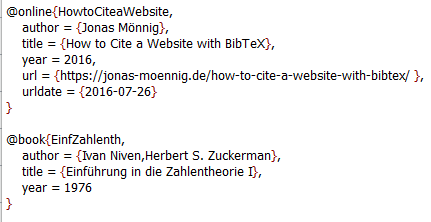
\includegraphics{Literatur}
\end{figure}\hfill\\
Direkt nach \textbf{\{} wird ein beliebiger Name für das Zitieren der Quelle festgelegt. Die erste Quelle kann also mit \glqq HowtoCiteaWebsite\grqq\, zitiert werden und die zweite mit \glqq EinfZahlenth\grqq.

Nachdem diese Datei erstellt ist, muss sie als Literatur in die .tex Datei eingefügt werden. Dies gelingt mit \textbf{\textbackslash addbibresource\{Literatur.bib\}}. Nun können die Zitate mit \textbf{\textbackslash cite\{Name der Quelle\}} zitiert werden.
Um die erste Quelle zu zitieren, nutzt man den Befehl \textbf{\textbackslash cite\{HowtoCiteaWebsite\}}. Damit erhalten wir folgendes Ergebnis:\\
\hspace*{0.5cm} Hier kommt ein Zitat aus der ersten Quelle \cite{HowtoCiteaWebsite}\\

\noindent Um noch die Seitenzahl zu spezifizieren, auf der das Zitat zu finden ist, fügt man [Seitenzahl] zwischen dem cite und \{ auf ein. Um also ein Zitat von Seite 12 aus der zweiten Quelle zu markieren, benutzt man \textbf{\textbackslash cite[12]\{EinfZahlenth\}}. Das Ergebnis sieht wie folgt aus:\\
\hspace*{0.5cm} Hier kommt ein Zitat von Seite 12 aus der zweiten Quelle \cite[12]{EinfZahlenth}\\
Will man noch ein f bzw. ff mit angeben fügt man ein \textbf{\textbackslash psq} bzw. \textbf{\textbackslash psqq} hinter der Zahl hinzu.\\
Weitere Infos zum Zitieren in \LaTeX\, finden sich auch diesen Webseiten:\\
\href{https://de.wikibooks.org/wiki/LaTeX-Kompendium:_Zitieren_mit_BibTeX}{https://de.wikibooks.org/wiki/LaTeX-Kompendium:\_Zitieren\_mit\_BibTeX}\\
\href{https://en.wikibooks.org/wiki/LaTeX/Bibliography_Management}{https://en.wikibooks.org/wiki/LaTeX/Bibliography\_Management}\\

Zitiert man zum ersten Mal eine neue Quelle, die man in der .bib Datei neu erstellt hat, muss man ein paar Schritte durchführen, um das Ergebnis in der erzeugten Datei zu sehen. Dafür öffnet man die .tex Datei in TeXworks, da TeXmaker die nötigen Befehle leider nicht unterstützt.
\begin{addmargin}{1.5cm}
\begin{itemize}
\item[Schritt 1] Oben links neben dem grünen Dreieck \glqq pdfLaTeX\grqq\, auswählen und anschließend das grüne Dreieck drücken.
\item[Schritt 2] Anstelle von \glqq pdfLaTeX\grqq\, nun \glqq Biber\grqq\, auswählen und anschließend das grüne Dreieck drücken.
\item[Schritt 3] Noch einmal Schritt 1 ausführen
\item[Schritt 4] Noch einmal Schritt 1 ausführen
\end{itemize}
\end{addmargin}
Nach diesen 4 Schritten sollte die Quelle in der generierten PDF Datei auftauchen.\\

\noindent Um das Literaturverzeichnis hinzuzufügen, benutzt man \textbf{\textbackslash printbibliography} an der gewünschten Stelle.



\chapter{Versionskontrolle mit GitHub}
Eine genaue Erklärung zur Versionskontrolle mit GitHub findet sich unter diesem Link \href{https://www.youtube.com/watch?v=85NjaDzec8U}{https://www.youtube.com/watch?v=85NjaDzec8U}  ab Minute 13.

%Literaturverzeichnis
\printbibliography


\end{document}